\documentclass[french]{article}

\usepackage[french]{babel}

\usepackage[utf8]{inputenc}
\usepackage[T1]{fontenc}
\usepackage[hidelinks,unicode]{hyperref}
\usepackage{graphicx}
\usepackage{amsmath}
\usepackage[left=1.3in,right=1.3in]{geometry}
\usepackage{microtype}
\usepackage{upquote}
\usepackage{csquotes}
\usepackage{url}
\usepackage[backend=biber]{biblatex}

\usepackage{tikz}
\usepackage{fontspec}

\usepackage{minted}
%\usemintedstyle{colorful}

\usepackage{pdfpages}

\usepackage{titling}
\newcommand{\subtitle}[1]{%
  \posttitle{%
    \par\end{center}
    \begin{center}\large#1\end{center}
    \vskip0.5em}%
}

\addbibresource{references.bib}

\title{Martine résout le problème du voyageur de commerce}
\subtitle{Avec un algorithme A*}
\author{Maxence \textsc{Aïci} \and Rémi \textsc{Nicole}}

\begin{document}

\maketitle

\tableofcontents

\part{Modélisation}

\paragraph{} Le problème du voyageur de commerce est probablement le problème
NP-complet le plus connu en algorithmique, mais dans le doute, voici la
définition de Wikipedia~\cite{wiki:tsp}:

\begin{quote}
	``Given a list of cities and the distances between each
	pair of cities, what is the shortest possible route that visits each city
	exactly once and returns to the origin city?''
\end{quote}

\paragraph{} Quant aux algorithmes de type A*, il s'agit tout simplement d'une
amélioration de l'algorithme de Dijkstra qui choisit sans aucun scrupule les
sommets qui sont le plus susceptible de nous mener à la solution optimale. On
calcule cette ``susceptibilité'' grâce à une heuristique qui calculera de
manière arbitraire une estimation du score restant pour aller à l'arrivée.

De manière mathématique, parce qu'en algorithmie, on aime bien écrire des
équations compliquées, et en plus en \LaTeX, ça nous donne un rendu magnifique:

\[f(n) = g(n) + h(n)\]

Avec:
\begin{itemize}
	\item $n$ l'étape par laquelle l'algorithme suggère de passer
	\item $f(n)$ l'estimation du coût total en passant par l'étape $n$
	\item $g(n)$ le coût d'aller du début jusqu'à l'étape $n$
	\item $h(n)$ l'estimation du coût pour aller de l'étape $n$ à l'arrivée
\end{itemize}

\section{Graphe de résolution de problème}

\paragraph{} Tout d'abords, il nous faut un arbre de résolution de problème
pour pouvoir faire de l'A*. Nous le définissons donc ainsi:

Si la carte des villes ressemble à ceci:
\begin{center}
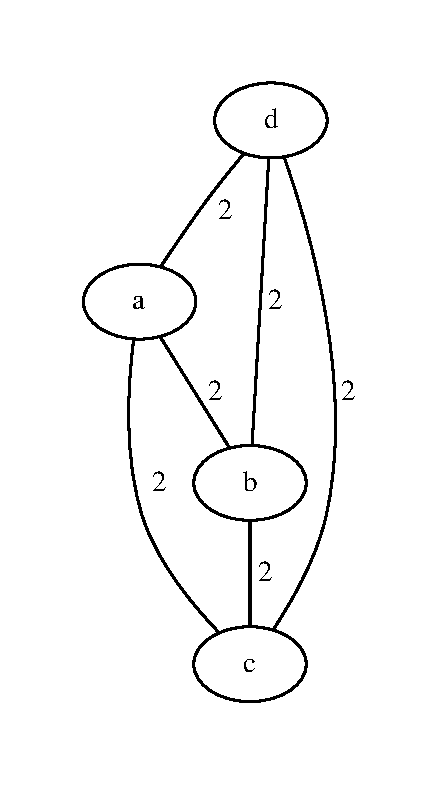
\includegraphics[scale=0.5]{graphs/modeling-the-problem_example1-map.pdf}
\end{center}

Alors on aura notre graphe de résolution de problème, ou PSG pour l'acronyme
anglais (aucune affiliation avec aucun groupe sportif), qui sera:
\begin{center}
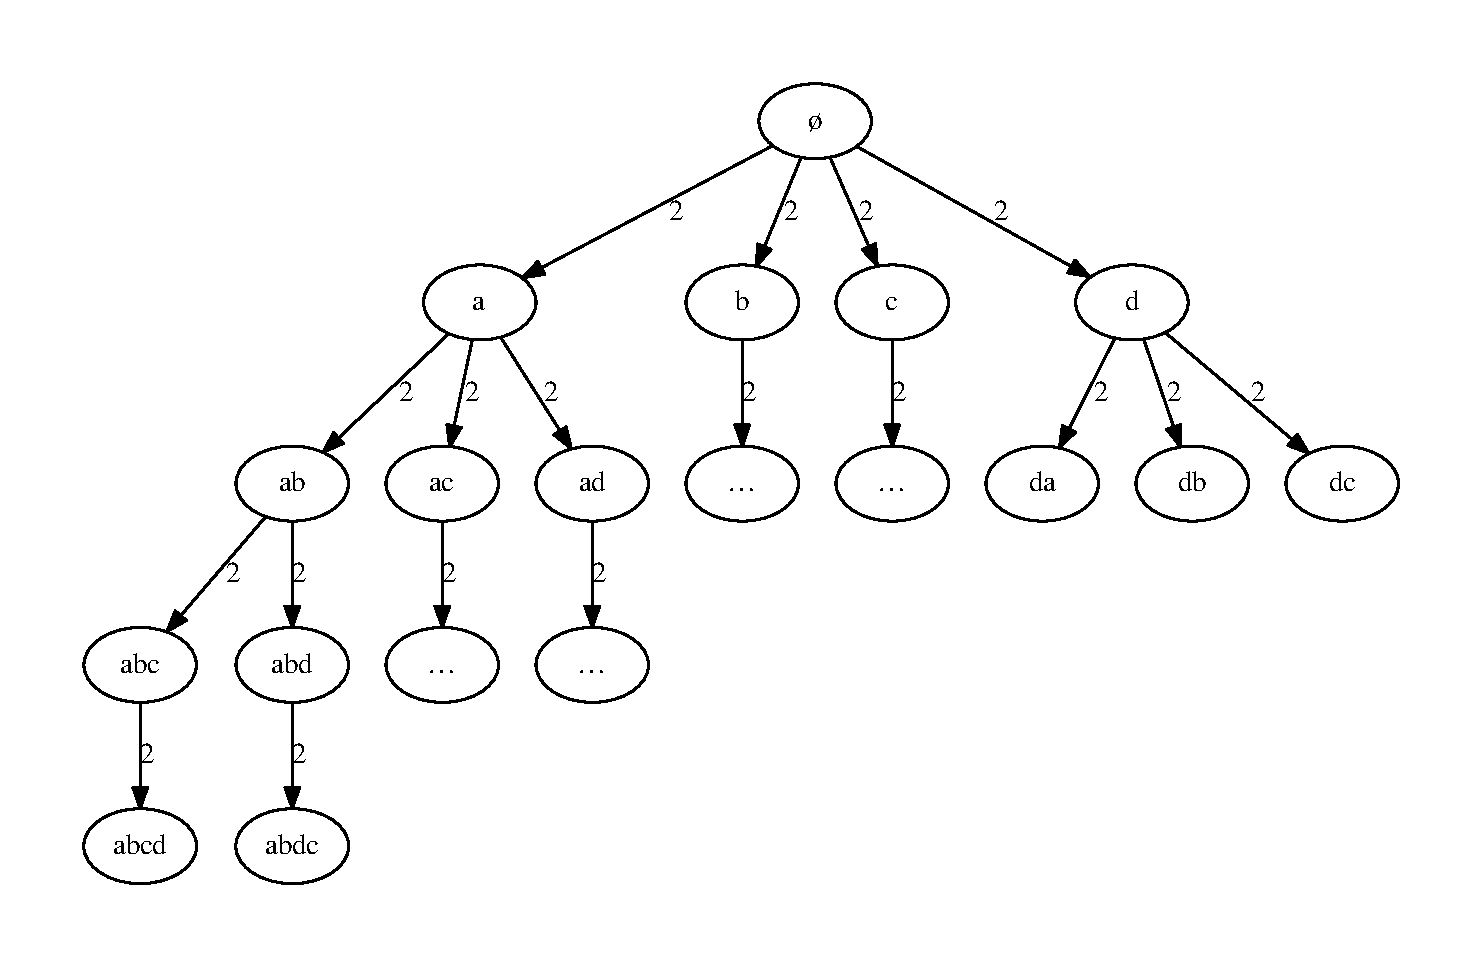
\includegraphics[scale=0.5]{graphs/modeling-the-problem_example1-psg.pdf}
\end{center}

Et, par exemple, après avoir pris le chemin A $\rightarrow$ B $\rightarrow$ C,
on aura:
\begin{center}
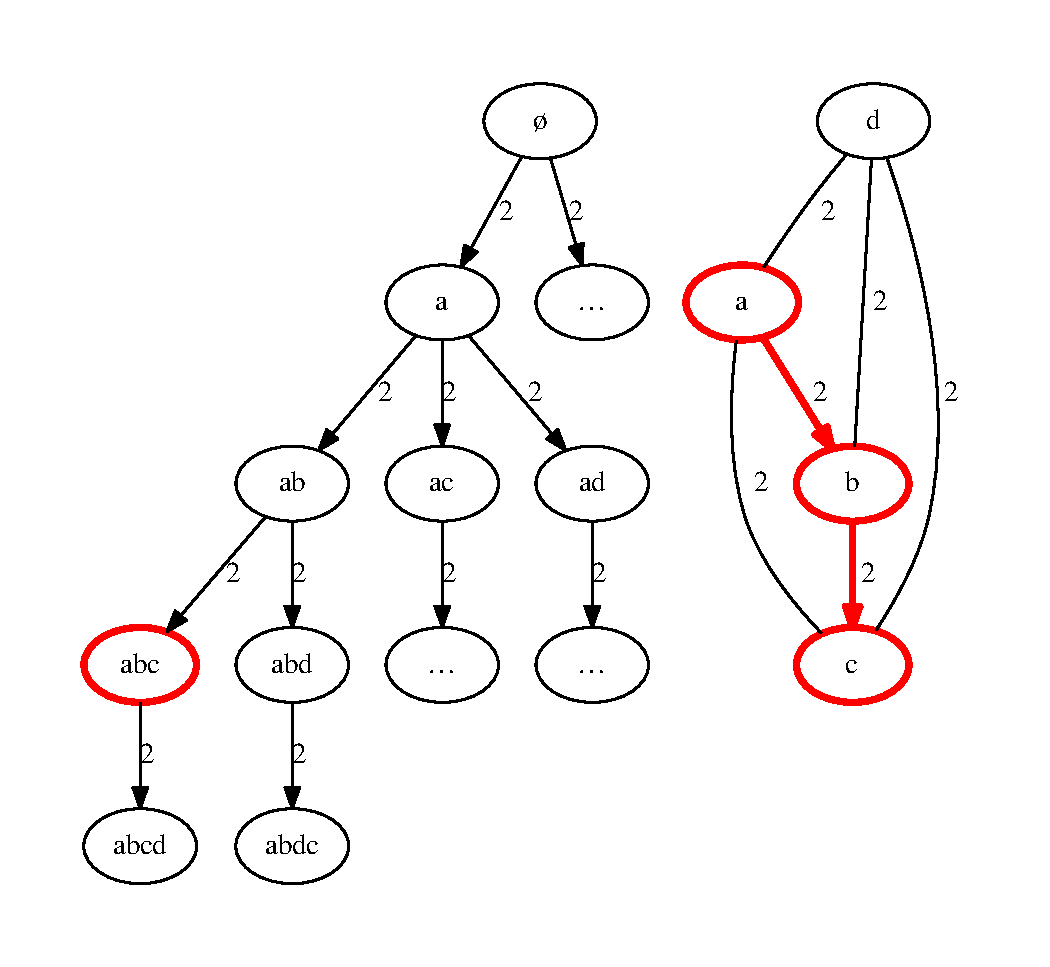
\includegraphics[scale=0.5]{graphs/modeling-the-problem_example2.pdf}
\end{center}

\section{Heuristiques}

\paragraph{} Pour ne pas être aussi inefficace que Dijkstra et pouvoir enfin
s'appeler A*, parce qu'avoir un nom prononçable c'est aussi important, il nous
faut des heuristiques. Il est aussi important d'avoir des heuristiques qui
estiment suffisamment bien le poids du chemin restant, mais tout en restant
facile à calculer parce que l'on risque d'en avoir souvent besoin au cours de
l'algorithme.

\subsection{Nulle}

\paragraph{} Comme son nom l'indique, l'heuristique nulle n'est pas terrible.
Il s'agit tout simplement de l'heuristique qui n'estime pas. En dehors d'être
le Saint Graal des heuristiques pour programmeurs fainéants, elle nous servira
aussi à tester notre algorithme, qui se ramènera donc à Dijkstra, ce qui m'a
fait reprendre à trois fois avant de pouvoir taper ce nom correctement. À
n'utiliser que en derniers recours, donc.

\subsection{Arête de poids minimum}

\paragraph{} Une autre heuristique simple, mais pas autant que précédemment,
est de prendre l'arête de poids minimum dans la carte privée des villes
parcourues, et de le multiplier par le nombre de villes restant à parcourir. Ce
n'est pas vraiment une bonne approximation, mais au moins on est sûr que le
chemin optimal aura comme borne inférieure le résultat de cette heuristique.

\subsection{Dijkstra}

\paragraph{} Curieuse coïncidence, on peut utiliser Dijsktra dans une
heuristique A*. Cette heuristique consiste à prendre le plus cours chemin de la
ville actuelle jusqu'à la ville de départ. Avec un peu de chance cette
approximation sera exacte, même si la complexité laisse à désirer.

\subsection{Arbre de poids minimum}

\paragraph{} Une utilisation intéressante de l'arbre de poids minimum, ou MST
pour l'acronyme anglais que l'on ne commentera pas, est de l'intégrer dans une
heuristique du voyageur de commerce. De plus, si l'on fait les bons choix
d'implémentation, il a une complexité de:

\[O(|\text{arêtes}| \times \log\left(|\text{sommets}|\right))\]

ce qui pourrait être un bon compromis entre la précision de l'approximation et
la complexité de l'heuristique.

Une fois que le MST de la carte, toujours privée des villes déjà parcourues,
est obtenu, il nous suffira de sommer le poids des arêtes et on aura notre
approximation!

\part{Outils}

\section{Moteur de production}

\begin{itemize}
	\item Meson~\cite{tools:meson} todo: dire que le site est moche
	\item Ninja~\cite{tools:ninja}
\end{itemize}

\textbf{\Huge{TODO}}

\section{Débogage}

\begin{itemize}
	\item gdb
	\item valgrind
	\item gprof
	\item Kcachegrind
\end{itemize}

\textbf{\Huge{TODO}}

\part{Implémentation des structures}

\paragraph{} Afin d'implémenter (ou d'implanter pour les gens bizarres) ces
types de graphes nous avons décidés de reprendre ce que j'avais\footnote{Ici
	Rémi qui parle} fait en C++ pour implémenter des algorithmes de l'unité
IT-3004 mais avait abandonnée au bout de deux jours parce que flemmingite
aigüe.

Nous avons donc développé par dessus un bout de code en C++ développé sur un
coup de tête, sans réflexion au préalable, et abandonné très rapidement. Aucun
moyen que cela tourne mal, donc.

\paragraph{} Il est important de préciser qu'au tout début du projet, nous
avions décidé d'utiliser la BGL (Boost Graph Library) pour implémenter par
dessus l'algorithme A*. Cependant, après beaucoup de frustration, de cheveux
perdus, et après avoir remarqué le manque de documentation, tutoriels ou
ressources en ligne, il était évidant que ce serait une chose à ne plus
refaire.

\section{État initial}

\subsection{Philosophie}

\paragraph{} Au tout début du projet, la partie graphe était seulement composée
de 4 classes: le graphe représenté par une liste d'adjacence, le graphe
représenté par une matrice d'adjacence, et leur classe ``d'itérateur évolué''
sur les sommets. Tous les graphes étaient orientés (et ils le sont toujours,
d'ailleurs)

\paragraph{} La classe de graphe représenté par une liste d'adjacence était
dans le namespace \texttt{list} et la classe de graphe représenté par une
matrice d'adjacence était dans le namespace \texttt{matrix}. L'idée était de
pouvoir faire:

\begin{minted}{cpp}
	using list::Graph;
	using list::Node;
	Graph myGraph;
\end{minted}

Ou l'équivalent avec \texttt{matrix} pour pouvoir choisir son type
d'implémentation. Même si, après rétrospection, ce n'était peut-être pas le
meilleur choix, cette philosophie est restée et a un peu évoluée au cours du
projet.

\subsection{Fonctionnalités}

\paragraph{} Au début du projet, voici ce qu'il était possibles de faire:

\begin{itemize}
	\item Construire un graphe directement avec une liste d'arcs:
		\begin{minted}{cpp}
	Graph myGraph{{1, 2}, {3, 4}, {1, 3}};
	Graph myGraph(4, {1, 2}, {3, 4}, {1, 3});
		\end{minted}
{\fontspec{Humor-Sans}
	\begin{tikzpicture}[overlay]
		\draw[thick,<-] (6:4.3) to [out=-30,in=180] (-2:8) [anchor=west,text width=2cm] node{Nombre de sommets};
	\end{tikzpicture}
}
	\item Ajouter des arcs.
	\item Calculer le symétrique du graphe.
	\item Calculer un composant connexe / fortement connexe du graphe.
	\item Compter le nombre d'arcs / de sommets.
	\item Opérer sur des connexions entre sommets:
		\begin{minted}{cpp}
	myGraph[1].isConnectedTo(3);
	myGraph[2].connectTo(4);
	myGraph[3].disconnectFrom(4);
		\end{minted}
\end{itemize}

\section{Évolutions}

\paragraph{} Il ne s'agit pas ici de parler de Pokémon, mais bien de
l'évolution du projet sur la partie implémentation des structures de graphes.
Quel dommage\ldots

\subsection{Refactorisations}

\paragraph{} Le projet a donc commencé de manière très agréable avec une série
de refactorisation du code de ce projet, afin de lui permettre d'être utilisée
pour faire des ``vrais'' algorithmes par dessus.

\paragraph{} Nous avons d'abords mis certaines fonctions hors des classes car
elle ne méritaient pas le status de ``méthodes''. Il s'agit surtout
d'algorithmes qui opèrent sur le graphe, comme le calcul de symétrique ou de
composantes connexes.

Afin de facilité le portage de ces fonctions et le développement de futurs
algorithmes, nous avons aussi rajouté des méthodes de parcours de sommets,
arcs, adjacents. Ces fonctions prennent en paramètre une fonction de rappel,
autrement appelé \emph{lambda} en C++, ce qui nous permets d'avoir un code
source clair et très joli à observer. Par exemple, pour l'algorithme du calcul
du symétrique, cela se résume à 4 lignes et un tiers:

\begin{listing}[H]
\begin{minted}{cpp}
Graph symmetric(Graph const& g) {
	Graph symmetricGraph;

	g.eachEdges([&symmetricGraph, &g](Node begin, Node end) {
		symmetricGraph.addEdges({end.getId(), begin.getId()});
	});

	return symmetricGraph;
}
\end{minted}
\caption{Un extrait de code aussi clair que net et précis}
\label{tsp:symmetric}
\end{listing}

\paragraph{} L'étape suivante à été de rajouter le type \texttt{ConstNode} qui,
à l'instar de la class \texttt{Node} permet d'accéder à des méthodes sur les
sommets uniquement, mais à partir d'un \texttt{Graph} non modifiable
(\mintinline{cpp}{const}). Pour éviter la duplication de code entre
\texttt{Node} et \texttt{ConstNode}, la solution choisie a été de créer une
classe mère \texttt{GenericNode} ayant un template pour pouvoir choisir si le
type des connexions internes est une référence ou une référence constante,
parce que \textbf{C++}!

\paragraph{} Puis, comme tout programmeur se doit de respecter les conventions
du langage, nous avons mis toutes les classe dans un namespace créé
spécialement pour l'occasion, que nous avons appelé \texttt{graph}, reflétant
notre nature d'adolescent engloutis par la société de consommation, délaissé
sans aucune originalité propre.

\paragraph{} Enfin, la plus grosse et donc la plus horrible des
refactorisations a été de permettre de pouvoir stocker des valeurs d'un types
arbitraires pour chaque sommet et pour chaque arc. Il a donc fallu rajouter un
double template aux classes \texttt{Graph}. Nous avons choisis de stocker ce
que l'on appellera les propriétés dans un vecteur pour les sommets, et dans une
map ayant pour clef une paire d'identifiant dans le cas des arcs. Il a fallu
ensuite concevoir une interface digne de ce nom. Nous avons aussi fournis des
structures pour des graphes avec des fonctionnalités basiques, comme par
exemple un poids ou, comme par hasard, des propriétés propre à l'A* ($g(n)$,
$h(n)$).

\part{Implémentation de l'algorithme}

Utilisation du namespace awesome, puis l'on démarrera notre propre
contre-culture.

\part{Tests}

\part{Jouer à Hercule Poirot}

\printbibliography%

\end{document}
